%%%%%%%%%%%%%%%%%%%%%%%%%%%%%%%%%%%%%%%%%%%%%%%%%%%%%%%%%%%%%%%%%%%%%%%%%%%%%%%%
\section{Discussion}
\label{sec:discussion}

%%%%%%%%%%%%%%%%%%%%%%%%%%%%%%%%%%%%%%%%%%%%%%%%%%%%%%%%%%%%%%%%%%%%%%%%%%%%%%%%
\subsection{A Time Reveresal WPT System}
\label{sec:system}

This research represents a first step in the exploration of building a
WPT system based on time reversal.
%
We demonstrate one possible realization of this idea in Fig.~\ref{fig:SysImage}.
%
However, we leave optimization of performance and efficiency to future work.


The proposed system consists of two basic components.
%
The first is a rectenna that serves as the receiver.
%
Although the system as described in Section~\ref{sec:meth} would require an
out-of-band feedback channel between the receiver and transmitter, prior work
has shown how a transmitter can target receivers entirely
in-band~\cite{nltr-wave-chaotic,roman}.
%
Our system in Fig.~\ref{fig:SysImage} builds on these findings.
%
The second is a transmitter that performs the time reversal process.
%
This component is responsible for recording characteristic signals from the
receiver(s), time reversing the signals, and re-broadcasting them into the
environment.



In a practical system, the rectenna could be integrated into the hardware of a
mobile device, or into an external component that plugs into the battery.
%
The transmitter would need to be connected to an external power source, but
could otherwise be located anywhere in the room.


Although not a component of the system, another important consideration in this
scenario is the environment; a low-loss scattering environment is necessary for
time reversal to be effective.
%%%%%%%%%%%%%%%%%%%%%%%%%%%%%%%%%%%%%%%%%%%%%%%%%%%%%%%%%%%%%%%%%%%%%%%%%%%%%%%%

\begin{figure}[t]
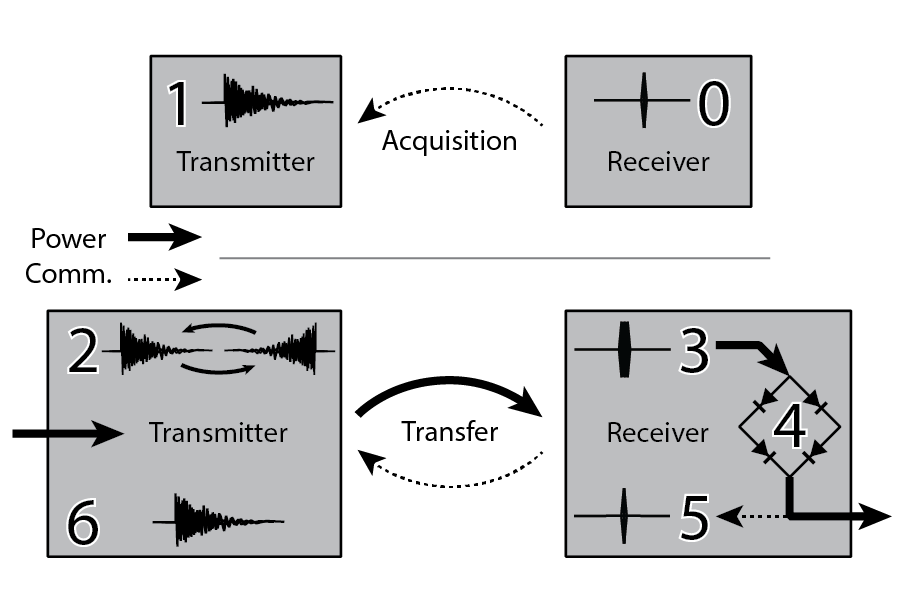
\includegraphics[width=\columnwidth]{figs/WPTSysAlt}
\caption{A notional time reversal WPT system. In the acquistion phase, a new receiver joins the system by broadcasting or emitting a characteristic signal (0). Here, the receiver actively emits a signal, but it is also possible for the transmitter to find a passive target, as shown in~\cite{nltr-wave-chaotic}. In either case, the next sona that the transmitter collects will contain spatial information unique to the receiver's location (1). In the power transfer cycle, the sona is time reversed (2), amplified, and broadcast back into the environment. The amplified signal reconstructs on the receiver (3) and is converted to usable DC power by the rectifier (4). A small fraction of the signal is used to re-broadcast a new characteristic signal (5) into the environment, which will be collected in the next sona (6). The cycle repeats from (2).}
\label{fig:SysImage}
\end{figure}

%%%%%%%%%%%%%%%%%%%%%%%%%%%%%%%%%%%%%%%%%%%%%%%%%%%%%%%%%%%%%%%%%%%%%%%%%%%%%%%%
\subsection{Limitations and Future Work}
\label{sec:contrib}

Our experiments were limited primarily by the environment and equipment used
in testing.
%
A consumer electronics environment is likely to be much larger than the chamber
used in this study, and filled with clutter.
%
Both of these properties would improve the modal density of the environment,
creating more transmission channels between source and target, ultimately
improving reconstruction quality.
%
On the other hand, such environments would likely create more loss.



In our experiments, we found that approximately 0.44\% of energy transmitted
through our test cavity was received.
%
Although this initial result is too low to act as the sole source of energy for
a device, it may be sufficient to perform long-term trickle charging or to act
as a secondary source of energy for extending battery life.
%
In order to improve efficiency, the most important area of future work would be
developing a better understanding of sources of environmental loss and how to
mitigate them.
%
In addition, our experiments used a single channel, but other WPT systems, such
as Cota, rely on a large number of channels~\cite{cota}.
%
Modifying the time reversal system to exploit multiple channels could improve
power transmission to levels sufficient for fully powering a device.



In Section~\ref{sec:moving}, we showed that the ability of a time reversal system
to transmit energy to a moving target is dependent on the spatial profile and
transmission dead time, $t_{d}$.
%
In this work, our equipment limited us to a $t_d$ of 7~seconds, which would be too slow
to handle most typical movement, such as walking across a room.
%
The primary bottlenecks here were the communication between the oscilloscope
and computer, and the fast Fourier transform (FFT) operations performed in MATLAB
on the computer.
%
A practical system could overcome these limitations by combining the two components
into a single device, which would remove the communication overhead, and optimizing for
the FFT computation in hardware.
%
Once a sona has been recorded (shown in Fig.~\ref{fig:sona} to be on the order of 10~$\mu$s),
the theoretical lower bound on processing time would be limited only by the amount of
time required to compute an FFT.
%%%%%%%%%%%%%%%%%%%%%%%%%%%%%%%%%%%%%%%%%%%%%%%%%%%%%%%%%%%%%%%%%%%%%%%%%%%%%%%%

%Nevertheless, we believe one of the main advantages of time reversal over
%existing WPT methods is its ability to adapt to moving targets without sacrificing
%range~\cite{fink,nltr-wave-chaotic}.